% Nallino, Part II p. 296: the ornamental rule that closes the notes on the tables, redrawn from the print at the size of
% the print (coordinates in pt from its centre, measured on a 300 dpi render): a thin rule 127 pt long with, in its
% middle, two swellings pointing outwards and an oval dot between them.
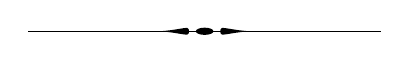
\begin{tikzpicture}[x=1pt,y=1pt]
\draw[line width=0.5pt] (-63.7,0) -- (63.7,0);
\foreach \s in {-1,1}
  \fill (16.2*\s,0) .. controls (11*\s,0.35) and (7.6*\s,1.3) .. (6.3*\s,1.2) .. controls (5.4*\s,1.1) and (5.4*\s,-1.1)
    .. (6.3*\s,-1.2) .. controls (7.6*\s,-1.3) and (11*\s,-0.35) .. cycle;
\fill (0,0) ellipse[x radius=3.2, y radius=1.3];
\end{tikzpicture}
